\chapter{Parte 1}
\label{cap:p1}

\section{Análise do problema}



Neste capítulo, pretende-se criar o modelo do caminho mais longo --- ou caminho
crítico ---, como um modelo de transportes em rede. No problema do caminho
crítico os nós correspondem atividades e a as arestas unidirecionais representam
as precedências entre atividades. Assim, a rede pode ser entendida como um
projeto, no qual as atividades devem ser realizadas obedecendo à ordem das
precedências. De notar que, o caminho mais longo é a duração mínima do projeto.


\begin{figure}[<+htpb+>]
	\centering
	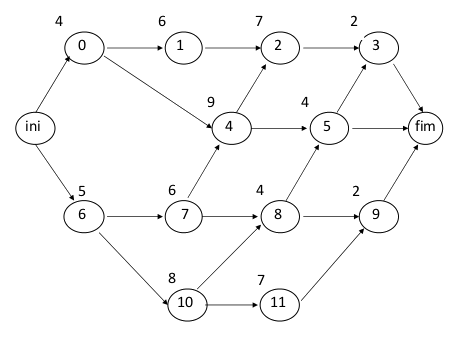
\includegraphics[scale=0.5]{./img/p1_rede_original}
	\caption{Grafo Inicial do enunciado}
\label{p1:fig:rede_original}
\end{figure}

Antes de partir para a formulação do modelo, foi necessário saber qual a rede
a considerar. À rede fornecida no enunciado (figura~\ref{p1:fig:rede_original})
foi necessário retirar dois nós, de acordo com a metodologia apresentada na
secção \textit{Determinação da Lista de Atividades} presente no final do
enunciado. O número de aluno do autor deste relatório é o nº 72628. Logo
o número mais alto é o 72628, então D=2 e E=8, sendo por isso os nodos
2 e 8 a ser retirados da rede. A rede resultante da remoção destes dois nós tem
a representação gráfica mostrada na figura~\ref{p1:fig:rede_com_duracoes}:

\begin{figure}[<+htpb+>]
	\centering
	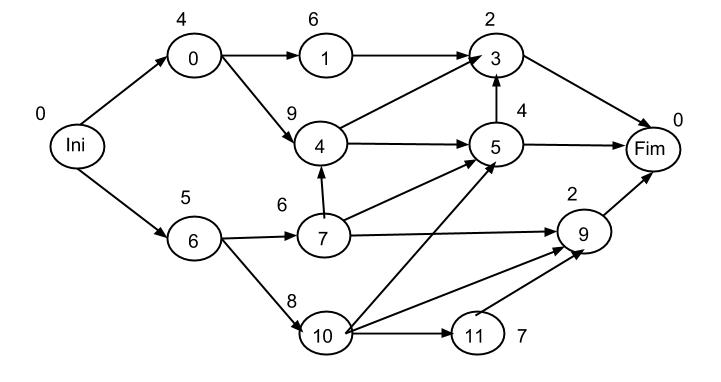
\includegraphics[scale=0.5]{./img/p1_rede_com_duracoes}
	\caption{Grafo resultante da remoção das atividades 2 e 8, com indicação da
	duração de cada atividade (em unidades de tempo arbitrárias)}
\label{p1:fig:rede_com_duracoes}
\end{figure}

\newpage
\section{Modelo}

\subsection{Parâmetros}

Os parâmetros deste modelo são as precedências e as durações de cada atividade,
bem como as capacidades do arco orientado, as ofertas e as procuras em cada
nodo.

\subsection{Variáveis de decisão}
\label{p1:subsec:vardec}


Como já se mencionou anteriormente pretende-se achar o caminho crítico do grafo
orientado. Cada arco terá um valor binário, i.e., 1 caso o arco faça parte do
caminho, 0 caso contrário, considerando que se injeta uma unidade de fluxo no
vértice inicial. Para o efeito, as variáveis de decisão serão nomeadas
$X_{I\_J}$ para a representação dos arcos, tal que a atividade I precede
a atividade J. Assim, $X_{2\_4}$ representa a aresta que vai da atividade 2 para
a atividade 4.

\subsection{Função objetivo}

No caminho mais longo em programação linear, a função objetivo é  uma expressão
que indica a duração de um caminho, onde se pretende que tome o maior valor
possível. Trata-se por isso de um problema de maximização.  Todavia neste
trabalho pretende-se achar o caminho crítico, modelando o problema como um
problema de transportes em rede, ou seja pretende-se minimizar o custo de
transporte, neste caso de uma unidade de fluxo da atividade inicial até à final,
satisfazendo a oferta e a procura em cada nó do grafo. Adiante nesta capítulo
esclarecer-se-á a transformação necessária do primeiro para o segundo modelo.

As variáveis de decisão indicam os arcos que fazem ou não parte de um caminho,
tanto num caso como no outro. A essas variáveis de decisão associaram-se os
custos de cada um dos arcos. Considerou-se que cada arco tem um custo associado
à origem desse arco. Por exemplo, o arco $X_{0\_1}$ tem origem na atividade
0 e destino na atividade 1, e terá um custo de 4, visto ser essa a duração da
atividade 0. Considera-se que a atividade não tem duração para efeitos práticos,
no entanto a passagem de uma atividade para outra passa a assumir a duração.


A função objetivo será o somatório de todos os custos de cada arco multiplicado
pela participação desse arco no caminho crítico. No modelo de programação
linear, para determinar a duração mínima, temos que:

\begin{displaymath}
\max~z = \sum  C_{I\_J} \times X_{I\_J}
\end{displaymath}

Onde:
\begin{description}
	\item[$C_{I\_J}$] Custo associado ao arco que vai de I para J --- parâmetro do problema
	\item[$X_{I\_J}$] Variável de decisão indicativa se o arco faz ou não parte do
	caminho, conforme detalhado na secção~\ref{p1:subsec:vardec}.
\end{description}

Para a transformação deste modelo num modelo de transportes em rede
considerou-se o uso do método simplex dual. A solução com este método
é simétrica da solução do simplex primal. Assim: 

\begin{displaymath}
	\max~z = \sum  C_{I\_J} \times X_{I\_J} \Leftrightarrow - \min -z = \sum
	- C_{I\_J} \times X_{I\_J}
\end{displaymath}




Expandindo a expressão e substituindo os valores de $C_{I\_J}$ pelos valores de
custos do enunciado, juntamente com as variáveis de decisão, temos a seguinte
expressão:

\begin{verbatim}
- min: - 0 Xini_0 - 0 Xini_6 - 4 X0_1 - 4 X0_4
     - 6 X1_3 - 2 X3_fim - 9 X4_3 - 9 X4_5
     - 4 X5_3 - 4 X5_fim - 5 X6_7 - 5 X6_10
     - 6 X7_4 - 6 X7_5 - 6 X7_9 - 2 X9_fim
     - 8 X10_5 - 8 X10_9 - 8 X10_11
     - 7 X11_9;
\end{verbatim}

\subsection{Restrições}
\label{p1:sec:restricoes}

No modelo de transportes em rede as restrições podem ser: restrições de
conservação de fluxo e restrições aos limites superiores e inferiores das
capacidades de cada arco. Dado que para este modelo se considera que uma unidade
de fluxo entra no nodo inicial e sai do nodo final, nada pode permanecer no
grafo, i.e., em cada nó o $fluxo~de~entrada = fluxo~de~saida$.

Assim temos que:

\begin{displaymath}
fluxo~entrada = fluxo~saida \Leftrightarrow  fluxo~entrada - fluxo~saida = 0
\end{displaymath}

Ao ter a equação escrita da segunda forma, considera-se implicitamente o fluxo
de entrada como sendo positivo e o fluxo de saída como negativo, neste caso
1 e -1.

Com a utilização do método simplex dual estas restrições veriam, todos os sinais
a inverterem-se. No entanto, como as todas as restrições são equações e não
inequações, não há nenhum efeito nestas pelo simplex dual. Ou seja, assumamos
o arcos fictícios $Xa\_b$ e $Xb\_c$, numa restrição também fictícia onde $Xa\_b
- Xb\_c = 0$. Com o método dual esta restrição fica como $-Xa\_b + Xb\_c = 0$,
que é equivalente a primeira. Assim $Xa\_b - Xb\_c = 0 \Leftrightarrow -Xa\_b
+ Xb\_c = 0$.

Estas restrições correspondem à procura e oferta em cada nó.

Dado que apenas entra e sai uma unidade de fluxo no grafo, a quantidade que
passa em cada arco será sempre um, pelo que não existe limite superior. Não
obstante, as restrições de não-negatividade serão sempre o limite inferior.

As restrições completas do modelo podem ser vistas na
secção~\ref{p1:sec:fichin}.


\section{Ficheiro \emph{Input}}
\label{p1:sec:fichin}
O ficheiro de \emph{input} é constituído pela função objetivo e restrições, detalhadas
em secções anteriores.

\begin{verbatim}
12                   
20                   
1    2     0     1000 
1    6     0     1000 
6    7    -5     1000 
6   10    -5     1000 
2    4    -4     1000 
2    3    -4     1000 
3    8    -6     1000 
4    5    -9     1000 
4    8    -9     1000 
5    8    -4     1000 
5   12    -4     1000 
7    4    -6     1000 
7    5    -6     1000 
7    9    -6     1000 
10   5    -8     1000 
10  11    -8     1000 
10   9    -8     1000 
11   9    -7     1000 
9   12    -2     1000 
8   12    -2     1000 
1                   
0                    
0                    
0                    
0                    
0                    
0                    
0                    
0                    
0                    
0                    
-1                    

\end{verbatim}

\newpage

\section{\emph{Output} produzido pelo \emph{Relax4}}

O \emph{output} apresentado a seguir foi obtido por \emph{copy-paste} direto
resultante da execução do \emph{Relax4} para
o ficheiro de \emph{input} apresentado anteriormente:

\begin{verbatim}
END OF READING
 NUMBER OF NODES = 12, NUMBER OF ARCS = 20
 CONSTRUCT LINKED LISTS FOR THE PROBLEM
 CALLING RELAX4 TO SOLVE THE PROBLEM
 ***********************************
 TOTAL SOLUTION TIME =  0. SECS.
 TIME IN INITIALIZATION =  0. SECS.
   1 6  1.
   6 7  1.
   4 5  1.
   5 8  1.
   7 4  1.
   8 12  1.
 OPTIMAL COST =  -26.
 NUMBER OF AUCTION/SHORTEST PATH ITERATIONS = 38
 NUMBER OF ITERATIONS =  12
 NUMBER OF MULTINODE ITERATIONS =  1
 NUMBER OF MULTINODE ASCENT STEPS =  0
 NUMBER OF REGULAR AUGMENTATIONS =  2
 ***********************************
\end{verbatim}

\newpage

\section{Resultado}

De acordo com o ficheiro de \emph{output} obtido, o caminho mais longo tem
a duração de 26 unidades de tempo e é o que passa pelas arestas $X_{ini\_6}$,
$X_{6\_7}$, $X_{7\_4}$, $X_{4\_5}$, $X_{5\_3}$ e $X_{3\_fim}$. Em termos
gráficos, o resultado é o apresentado na figura~\ref{p1:fig:caminho_critico}. As
setas de linha cheia indicam as arestas que fazem parte do caminho mais longo,
e os nós por onde esse caminho passa foram colocados a verde.

\begin{figure}[<+htpb+>]
\centering
		  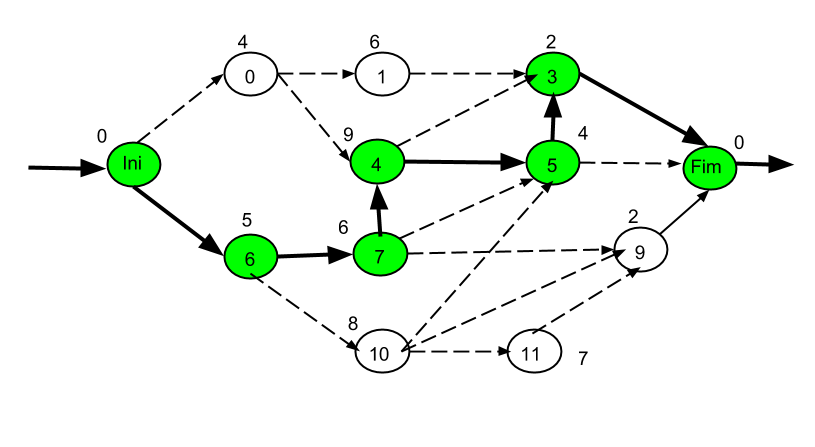
\includegraphics[scale=0.5]{./img/p1_caminho_critico}
\caption{Grafo com indicação do caminho crítico obtido. Os valores em cada nó
representam a duração (em unidades de tempo) da respetiva atividade}
\label{p1:fig:caminho_critico}
\end{figure}

Este resultado indica que as atividades 6,7,4,5 e 3 devem ser vigiadas de perto
e deve-se tentar garantir que são executadas nos tempos previstos, sem atrasos,
caso contrário todo o projeto será atrasado.

\section{Validação do Modelo}

Para validar os resultados, tanto na função objetivo como nas restrições,
substituímos os valores das variáveis de decisão pelo valor que estas tomam na
solução que o lp\_solve indica como ótima. A ideia é verificar que os valores
das variáveis de decisão obtidos confirmam o valor da função objetivo obedecendo
a todas as restrições.

Para evitar ao máximo o erro humano, a substituição de variáveis foi feita
recorrendo a ferramentas que auxiliaram a substituição automática das variáveis
pelo seu valor.

\subsection{Variáveis de Decisão}

No resultado obtido todas as variáveis são de facto binárias, tomam apenas
o valor de 0 ou 1, tal como esperado.

\subsection{Função objetivo}

Depois da substituição das variáveis pelo seu valor, a função objetivo
fica:\\[0.5cm]

$0*0+0*1+4*0+4*0+6*0+2*1+9*0+9*1+4*1+4*0+5*1
+5*0+6*1+6*0+6*0+2*0+8*0+8*0+8*0+7*0 = 26$\\[0.5cm]

Inserindo a expressão numa calculadora verifica-se que a expressão é igual a 26,
o que confirma o resultado obtido com o \textit{lp\_solve}.

\subsection{Restrições}

\begin{itemize}

\item Nodo Inicio 

$1-X_{ini\_6} - X_{ini\_0} = 0$

$1 - 1 - 0 = 0$

\item Nodo 0 

$X_{ini\_0}-X_{0\_1}-X_{0\_4} = 0$

$0 - 0 - 0 = 0$

\item Nodo 1 

$	X_{0\_1}-X_{1\_3} = 0$

$0 - 0 = 0$

\item Nodo 3 

$	X_{1\_3} + X_{4\_3} + X_{5\_3}-X_{3\_fim} = 0$

$0 + 0 + 1 - 1 = 0$

\item Nodo 4 

$	X_{0\_4} + X_{7\_4} - X_{4\_3} - X_{4\_5} = 0$

$0 + 1 - 0 - 1= 0$

\item Nodo 5 

$X_{4\_5} + X_{7\_5} + X_{10\_5} - X_{5\_3} - X_{5\_fim} = 0$

$1 + 0 + 0 - 1 - 0 = 0$

\item Nodo 6 

$X_{ini\_6} - X_{6\_7} - X_{6\_10} = 0$

$1 - 1 - 0 = 0$

\item Nodo 7 

$X_{6\_7}- X_{7\_4}- X_{7\_5} - X_{7\_9} = 0$

$1 - 1 - 0 - 0 = 0$

\item Nodo 9 

$X_{7\_9} + X_{10\_9} + X_{11\_9} - X_{9\_fim} = 0$

$0 + 0 + 0 - 0 = 0$

\item Nodo 10 

$X_{6\_10} - X_{10\_5} - X_{10\_9} - X_{10\_11} = 0$

$0 - 0 - 0 - 0 = 0$

\item Nodo 11 

$X_{10\_11} - X_{11\_9} = 0$

$0 - 0 = 0$

\item Nodo Fim 

$X_{3\_fim} + X_{5\_fim} + X_{9\_fim} - 1 = 0$

$1 + 0 + 0 - 1 = 0$

\end{itemize}

Assim conclui-se que todas as restrições são respeitadas.







